\documentclass[aspectratio=169]{beamer}
\usepackage[english]{babel}
\usepackage[utf8]{inputenc}

% AMSLaTeX packages
\usepackage{amsthm}
\usepackage{amsmath}
\usepackage{amsfonts}
\usepackage[algoruled]{algorithm2e}

\usetheme{default}
\useoutertheme{default}
% we want to use images
\usepackage{graphicx}
\usepackage{movie15}
\usepackage{hyperref}

% table relates packages
\usepackage{booktabs}
\usepackage{multirow}
% pick a font
\usepackage{palatino}           
% \usepackage{times}
\usepackage{tikz}
\usetikzlibrary[positioning,arrows,decorations.pathmorphing,backgrounds,fit,calc]
% \AtBeginSection[]  % "Beamer, do the following at the start of every section"
% {
%   \begin{frame}<beamer> 
%     \frametitle{Outline} % make a frame titled "Outline"
%     \tableofcontents[currentsection]  % show TOC and highlight current section
%   \end{frame}                    
% }

% \AtBeginSubsection[]
% {
%   \begin{frame}
%     \frametitle{Outline}
%     \tableofcontents[currentsection,currentsubsection]
%   \end{frame}
% }

\AtBeginSection[]
{
   \begin{frame}
       \frametitle{Outline}
       \tableofcontents[currentsection]
   \end{frame}
}

\newcommand{\ebox}[1][1em]{\framebox[#1]{\phantom{M}}}

\setlength\arraycolsep{1.4pt}% some length

%gets rid of navigation symbols
\setbeamertemplate{navigation symbols}{}

%gets rid of bottom navigation bars
\setbeamertemplate{footline}[page number]{}
\setbeamertemplate{headline}{}


\usebackgroundtemplate{
\includegraphics[width=\paperwidth]{../templates/NormalANLBlue}}
\title{Multiobjective Optimization of Simulations with PARMOO}
\author{Tyler Chang$^a$ and Stefan Wild$^a$}
\institute{$^a$Mathematics and Computer Science Division,\\
Argonne National Laboratory}
\date{ANL Postdoctoral Research and Career Symposium\\November 3--10, 2020}
\begin{document}

\setbeamertemplate{footline}{}
{
\usebackgroundtemplate{
\includegraphics[width=\paperwidth]{../templates/TitleANLBlue}}
\frame{\titlepage}
}

\setbeamertemplate{footline}[page number]{}

% FRAME: overview
%\begin{frame}
%  \frametitle{Outlines}
%  \tableofcontents
%\end{frame}
% ========================================
% main slides come here
% ========================================
\begin{frame}\frametitle{What is Multiobjective Optimization?}
{\bf Problem setting:}\\
\medskip
\begin{columns}
\begin{column}{.3\textwidth}
We can control input variables...
\end{column}
\begin{column}{.25\textwidth}
We can observe the response to inputs...
\end{column}
\begin{column}{.3\textwidth}
We want to minimize quantities of interest...
\end{column}
\end{columns}
\begin{columns}
\begin{column}{.35\textwidth}
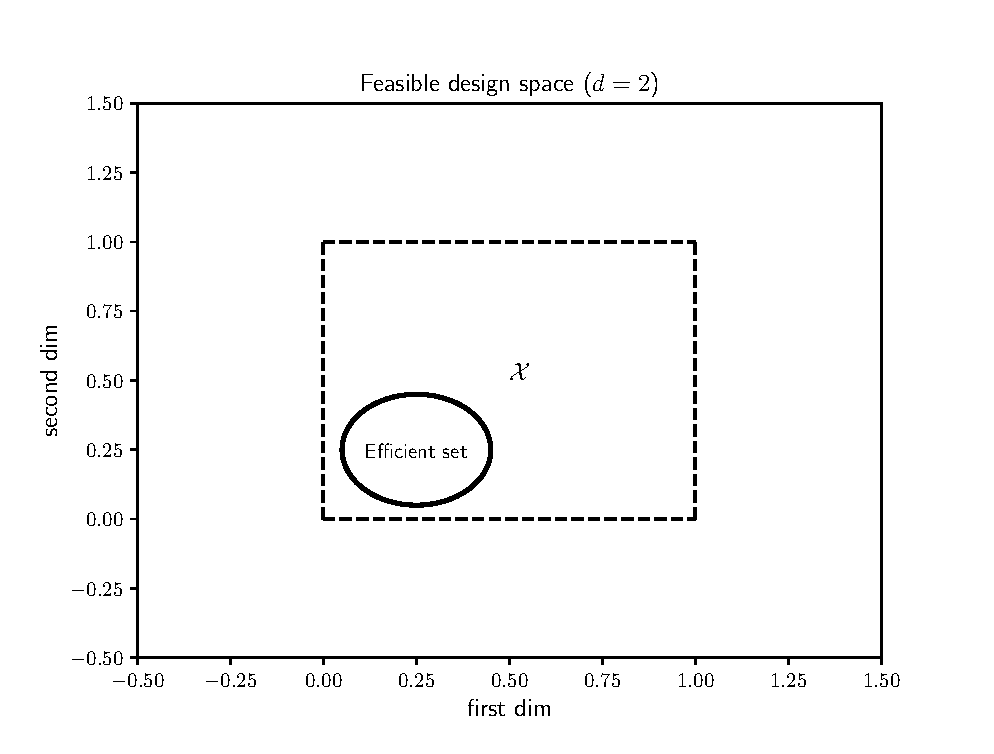
\includegraphics[width=\textwidth]{feasible_design.eps}
\end{column}
\begin{column}{.2\textwidth}
\begin{center}
{\scriptsize
Numerical simulation?\\
Real-world experiment?\\
Build a prototype?\\
Run a test?\\
}
$\xrightarrow{\hspace*{2cm}}$
$$
F : {\cal X} \rightarrow {\cal Y}
$$
\end{center}
\end{column}
\begin{column}{.35\textwidth}
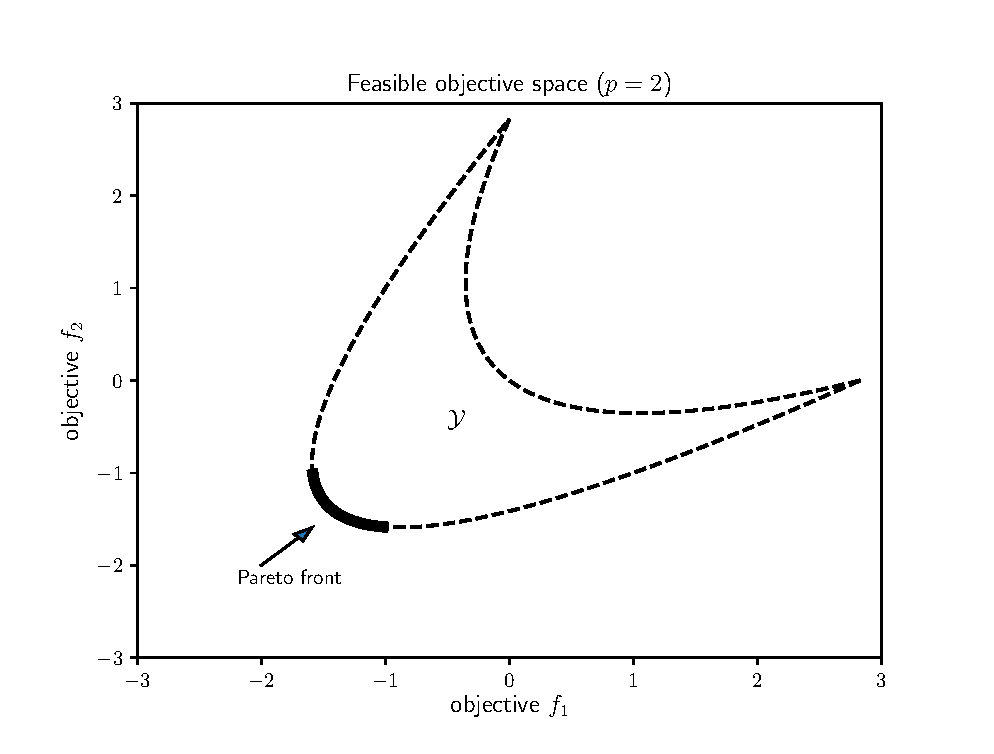
\includegraphics[width=\textwidth]{convex_pareto.eps}
\end{column}
\end{columns}
\medskip
Solution is the {\it Pareto front} --- a tradeoff surface balancing
conflicting objectives.
\end{frame}

\begin{frame}\frametitle{An Example in HPC System Performance}
Want to manage tradeoff between performance variability and mean
performance in {\tt HPL} linear system solver on HPC system {\tt Bebop} 
at Argonne
{\small
\begin{columns}
\begin{column}{.3\textwidth}
\begin{itemize}
\item Adjust 5 configuration settings for {\tt HPL}
\item For each setting, run {\tt HPL} 30 times on 4 nodes of {\tt Bebop},
and compute the mean and standard deviation of throughputs
\end{itemize}
\end{column}
\begin{column}{.2\textwidth}
\begin{center}
Use multiobjective optimization to maximize mean
\& minimize std dev
$$\xrightarrow{\hspace*{2cm}}$$
\end{center}
\end{column}
\begin{column}{.4\textwidth}
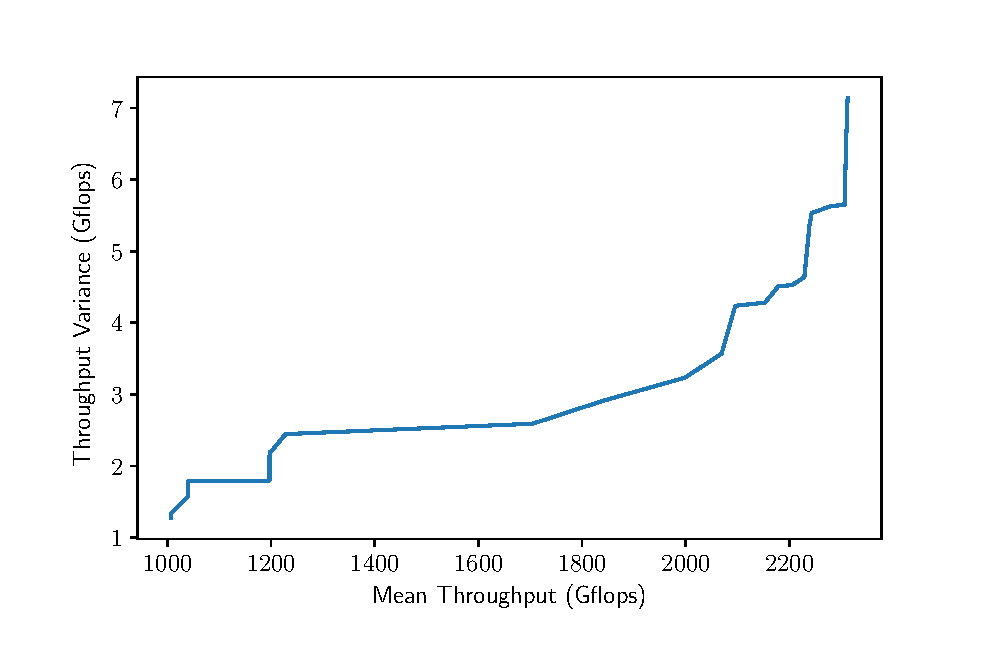
\includegraphics[width=\textwidth]{hpl_n20k_pf.eps}
\end{column}
\end{columns}
}
\medskip
{\tiny\it
[1] Chang, Larson, and Watson.
Multiobjective optimization of the variability of the high-performance 
LINPACK solver.
To appear in Proc.\ 2020 Winter Simulation Conference.\\
}
\end{frame}

\begin{frame}\frametitle{The Spectrum of Computational Expense}
\begin{columns}
\begin{column}{.3\textwidth}
\begin{center}
Reasonable!
\end{center}
\end{column}
\begin{column}{.3\textwidth}
\end{column}
\begin{column}{.3\textwidth}
\begin{center}
Very hard!
\end{center}
\end{column}
\end{columns}
\bigskip
\begin{columns}
\begin{column}{.3\textwidth}
\begin{itemize}
\item Eval: $\approx$ secs
\item Budget: $\approx 10,000$
\item Software: Genetic algorithms
\end{itemize}
\end{column}
\begin{column}{.3\textwidth}
\begin{itemize}
\item Eval: $\approx$ mins
\item Budget: $\approx 1000$
\item Software: Research codes
\end{itemize}
\end{column}
\begin{column}{.3\textwidth}
\begin{itemize}
\item Eval: $\approx$ hrs
\item Budget $\approx 100$
\item Software: ??
\end{itemize}
\end{column}
\end{columns}
\bigskip
Computationally cheap $\xrightarrow{\hspace*{7cm}}$ expensive
\end{frame}

\begin{frame}\frametitle{PARMOO}
Our solver is PARMOO --- A flexible framework for solving multiobjective
optimization problems all accross the expense spectrum
\begin{itemize}
\item In order to solve problems of varying expenses and with varying
amounts of available domain knowledge, we support interchangable solvers,
search strategies, problem types, and varying amounts of information
\item We will also leverage the {\tt libEnsemble} library for extreme
scale parallelism
\end{itemize}
\end{frame}

\begin{frame}\frametitle{Continued Work}
\begin{itemize}
\item We are working on adding solvers and features to support widening classes
of problems
\item We are also looking into the integration with {\tt libEnsemble} [2]
\item We are looking for new problems to test our solvers on and
and widen our support for new problem types!
\end{itemize}
\medskip
{\tiny\it [2]
Chang, Larson, Watson, and Lux.
Managing computationally expensive blackbox multiobjective optimization
problems with libEnsemble.
In Proc. 2020 Spring Simulation Conference (SpringSim '20).
SCS, Fairfax, VA, USA, Article No. 31, 12 pages.\\
}
\end{frame}

\begin{frame}\frametitle{Questions}
\begin{center}
{\huge
Email: tchang@anl.gov\\
\bigskip
BlueJeans Q\&A Room:  580 115 580
{\large (\url{https://bluejeans.com/580115580})}}\\
\bigskip
\bigskip
\bigskip
{\small This material is based upon work supported by the U.S. Department of Energy, Office of Science, Office of Advanced Scientific Computing Research, SciDAC program under contract number DE-AC02-06CH11357.}
\end{center}
\end{frame}

\end{document}
